Question:\\
\emph{
    Web exercise:
- Recommend a DW DBMS for the Census Bureau.\\\\ The list is open, but examples
are PostgreSQL, CockroachDB, TiDB, SingleStore MemSQL and ClickHouse.\\ Your
recommendation should be based on five criteria. You are supposed to score
three vendors. Scoring should be based on data you collect from web sources.
See below hint:}\\

Kim-input: A list with 10 different criteria for (or features of) DW DBMS is presented in 
the lecture notes. \footnote{See document: 00 DBII-Part II-2025-AE, p.11} 

\begin{figure}[h] % "h" means "here"
    \centering
    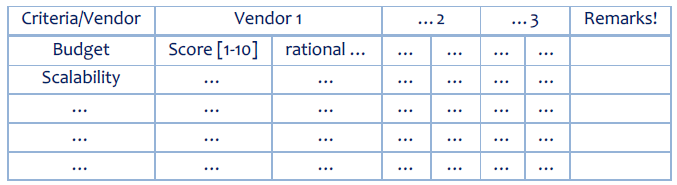
\includegraphics[width=0.5\textwidth]{Figures/Q7_QUESTION_table.PNG}
    \label{fig:my_image}
\end{figure}

\emph{[00:15:13] question number seven that's a web exercise and and i have talked about that
um in the beginning of the lectures so i recommend a data warehouse engine so a dbms engine for the
census office of course if you google you will um the term i mean what is the data warehouse engine used
for example by the swedish census office or finnish or us or german or etc they all are using by the way
and then you will get some uh case studies telling yeah those are using for example oracle technology
those are using pulse to grass and those are using teradata and yeah uh green plum and a lot of names
it's only uh some names that i have put here so so that the question here that i want to
yeah uh like test your ability to compare and recommend the technology so the name is not important so for
once again there is no model answer here to the name so for example if you ended up saying it's a tie db
and somebody else said no it's a single store and third student said it's a click house you all might
be right yeah as long as you have evaluated those options and put a criteria this is an exercise on
evaluation rather than an exercise on selection uh can we evaluate yeah what are the evaluation criteria
i put examples here like scalability and i talked about scalability in the course
or budget which one is cheaper uh yeah or which one is most expensive usually the cheapest gets the
highest points and the most expensive gets the lowest points when it comes to the budget criteria
which one is a scalable horizontal and vertical and we have talked about this and so forth so so you need
to collect the data um and compare}\\

What to do here?
\begin{enumerate}
    \item Choose three vendors
    \item Choose 5 criteria
    \item Evaluate each vendor in each criteria (in a table, see question)
    \item Summarize and recommend a DW DBMS for Census Bureau
  \end{enumerate}
\newpage Answers to Question 7:
testref \cite{benchmark}
\section{The Web Exercise}
This question requires a web exercise,therefore we have decided to add sections, one for each product. 

\subsection{Choice of criteria:}
The criteria we have chosen to evaluate the vendors and why are:
\begin{itemize}
    \item Scalability: This is an important criteria since:
    \begin{quotation}
        "Can we scale up, so this is important [...] the goverment is opening up it's database to the public for example.[...] so scalable means it can support more users and larger data volume"\cite[t.00:53:00]{l1video}".
    \end{quotation}
    \item Storage: Storage is an important criteria since
    the DBMS must efficiently handle large volumes of data, 
    ensuring optimal load performance and storage management to 
    accommodate growing datasets without architectural limitations \cite[p. 1239]{CourseLitt}.
    \item Cost: This is an important criteria since developing a DBMS is a costly endeavour, and the cost of the chosen DBMS can add or substract from this. \begin{quotation}
        "the cost can vary enormously from tens of thousands to millions of dollars due to
    the variety of technical solutions available." \cite[p. 1226]{CourseLitt}
    \end{quotation}
    \item Security: \begin{quote}
        "Security is critical to the data warehouse. To provide the strongest possible
security and to minimize administrative overhead, all security policies are enforced
within the data warehouse."\cite[p. 1309]{CourseLitt}
    \end{quote}
    \item Latency: This is an important criteria since \begin{quotation}
         "the DBMS must be able to handle large, complex queries for key business operations that must complete in reasonable time periods." \cite[p. 1239]{CourseLitt}
    \end{quotation} 
\end{itemize}
\subsection{Vendor 1 - ClickHouse:}
    
\subsection{Vendor 2 - SingleStore:}
    
\subsection{Vendor 3 - PostgreSQL:}

\section{The Comparison}
In this section we provide a comparison between vendors, therefore we have decided to add sections, one for each criterion. 

\subsection{Criteria 1 - Scalability:}
 
\subsection{Criteria 2 - Storage:}

\subsection{Criteria 3 - Cost:}

\subsection{Criteria 4 - Security:}

\subsection{Criteria 5 - Latency:}
